% !TEX root = knottedMain.tex
\documentclass[varwidth=\maxdimen]{standalone}

\usepackage{mathtools,amssymb,mathrsfs,dutchcal,upgreek,faktor,accents,etoolbox,multicol}
\usepackage[dvipsnames]{xcolor}
\definecolor{mygreen}{RGB}{	8,156,79 }
\usepackage{tikz,tikz-cd}
\usetikzlibrary{patterns,knots,arrows.meta,decorations.markings}
\tikzset{>={Straight Barb[scale=0.85]}}
\tikzcdset{
  cells={font=\everymath\expandafter{\the\everymath\displaystyle}},
  arrow style=tikz,
  diagrams={>={Straight Barb[scale=0.85]}},
  every label/.append style = {font = \small}
}


\begin{document}
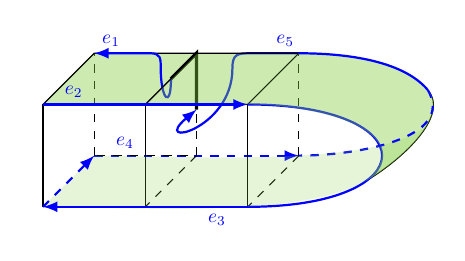
\begin{tikzpicture}[scale=1.3,every node/.style={scale=0.7}]
\clip (-0.9,-1) rectangle (3.1,1);

    \draw[blue,thick,-latex,dashed]
        (-0.25,-0.25) -- (1.75,-0.25) node[above,pos=0.15]{$e_4$};

% ext region for B_1
    \draw[dashed]
        (-0.25,-0.25) rectangle (0.75,0.75);


    \fill[yellow!45!green!90!white,fill opacity=0.4,draw=black]
        (-0.75,0.25) -- (0.25,0.25) -- 
        (0.75,0.75) -- (-0.25,0.75) -- (-0.75,0.25);

    \fill[yellow!45!red,fill opacity=0,draw=black]
        (-0.75,-0.75) rectangle (0.25,0.25);

    \draw[very thick] (0.75,0.2) -- (0.75,0.75) -- (0.5,0.5) ;
% B_2
    \draw 
        (2.4, -0.5) to[out=30,in=-50,distance=0.35cm] (3.01,0.39);

    \draw[blue,thick,latex-] 
        (0.75,0.2)  
        to[out=-140,in=-90,distance=0.6cm]
        (1.1,0.6) to[out=90,in=180,distance=0.15cm]
        (1.3,0.75) -- (1.75,0.75) node[above,pos=0.7]{$e_5$} ; 
    \draw[blue,thick,-latex] 
        (0.5,0.5) to[out=-90,in=-90,distance=0.3cm] 
        (0.4,0.6) to[out=90,in=0,distance=0.1cm]
        (0.3,0.75) -- (-0.25,0.75) node[above,pos=0.7]{$e_1$} ; 

% ext region for B_2
    \draw[dashed]
        (1.75,-0.25) -- (1.75,0.75);
    \draw[dashed]
        (0.25,-0.75) -- (1.25,-0.75) -- 
        (1.75,-0.25) (0.75,-0.25) -- (0.25,-0.75);

    \fill[yellow!45!green!90!white,fill opacity=0.4,draw=black]
        (0.25,0.25) -- (1.25,0.25) -- 
        (1.75,0.75) -- (0.75,0.75) -- (0.25,0.25);

    \fill[green!45!red,fill opacity=0,draw=black]
        (0.25,-0.75) rectangle (1.25,0.25);
        
% front of B_2
    % \fill[yellow!45!green!90!white,fill opacity=0]
    %     (1.25,0.25) to[out=0,in=0,distance=1.75cm] (1.25,-0.75) -- (1.25,0.25);
    \draw[blue,thick]
        (1.25,0.25) to[out=0,in=0,distance=1.75cm] (1.25,-0.75);
    \fill[yellow!45!green!90!white,fill opacity=0.4]
        (1.75,0.75) to[out=0,in=130,distance=0.4cm] 
        (3.01,0.39) to[in=30,out=-50,distance=0.35cm] 
        (2.4, -0.5) to[out=40,in=0,distance=0.72cm] 
        (1.25,0.25) -- (1.75,0.75) ;
    \draw[blue,thick]
        (1.75,0.75) to[out=0,in=130,distance=0.4cm] 
        (3.01,0.39) ;
    \draw[dashed,blue,thick]
        (3.01,0.39)  to[out=-60,in=0,distance=0.55cm] (1.75,-0.25);

     \fill[yellow!45!green!90!white,fill opacity=0.2]
        (3.01,0.39)  to[out=-60,in=0,distance=0.95cm] (-0.25,-0.25)
        -- (-0.75,-0.75) to[out=0,in=-150,distance=0.75cm]  (2.4, -0.5) to[out=30,in=-50,distance=0.35cm]  (3.01,0.39) ;


    \draw[blue,thick,-latex]
        (-0.75,0.25) -- (1.25,0.25) node[above,pos=0.15]{$e_2$};
    \draw[blue,thick,-latex]
        (1.25,-0.75) -- (-0.75,-0.75) node[below,pos=0.15]{$e_3$};
    \draw[blue,thick,-latex,dashed]
        (-0.75,-0.75) -- (-0.25,-0.25) ;

\end{tikzpicture}
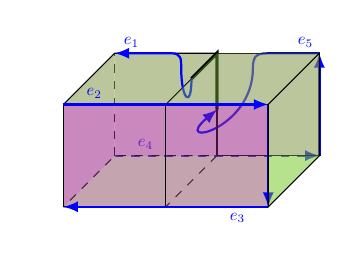
\begin{tikzpicture}[scale=1.3,every node/.style={scale=0.6}]
\clip (-1.1,-1) rectangle (1.9,1);

    \draw[blue,thick,-latex,dashed]
        (-0.25,-0.25) -- (1.75,-0.25) node[above,pos=0.15]{$e_4$};
    \draw[blue,thick,-latex]
        (1.75,-0.25) -- (1.75,0.75);

% ext region for B_1
    \fill[blue!45!red!80!white,fill opacity=0.3,draw=black,dashed]
        (-0.25,-0.25) rectangle (0.75,0.75);
    \fill[yellow!45!green!90!white,fill opacity=0.3,draw=black,dashed]
        (-0.75,-0.75) -- (0.25,-0.75) -- 
        (0.75,-0.25) -- (-0.25,-0.25) -- (-0.75,-0.75);
    \fill[blue!45!red!80!white,fill opacity=0.3]
        (-0.75,-0.75) -- (-0.75,0.25) -- (-0.25,0.75)-- (-0.25,-0.25) ; 
    \fill[yellow!45!green!90!white,fill opacity=0.4,draw=black]
        (-0.75,0.25) -- (0.25,0.25) -- 
        (0.75,0.75) -- (-0.25,0.75) -- (-0.75,0.25);
        

    \fill[blue!45!red!80!white,fill opacity=0.4,draw=black]
        (-0.75,-0.75) rectangle (0.25,0.25);

    \draw[very thick] (0.75,0.2) -- (0.75,0.75) -- (0.5,0.5) ;
% B_2
    \draw[blue,thick,latex-] 
        (0.75,0.2)  
        to[out=-140,in=-90,distance=0.6cm]
        (1.1,0.6) to[out=90,in=180,distance=0.15cm]
        (1.3,0.75) -- (1.75,0.75) node[above,pos=0.7]{$e_5$} ;
    \draw[blue,thick,-latex] 
        (0.5,0.5) to[out=-90,in=-90,distance=0.3cm] 
        (0.4,0.6) to[out=90,in=0,distance=0.1cm]
        (0.3,0.75) -- (-0.25,0.75) node[above,pos=0.7]{$e_1$} ; 

% ext region for B_2
    \fill[yellow!45!green!90!white,fill opacity=0.3]
        (1.25,-0.75) -- (1.75,-0.25) -- (0.75,-0.25) -- (0.25,-0.75);
    \fill[blue!45!red!80!white,fill opacity=0.3,draw=black]
        (0.75,-0.25) rectangle (1.75,0.75);

    \fill[yellow!45!green!90!white,fill opacity=0.4]
        (0.25,0.25) -- (0.75,0.75) -- 
        (1.75,0.75) -- (1.25,0.25) -- (0.25,0.25);

    \fill[blue!45!red!80!white,fill opacity=0.4,draw=black]
        (0.25,-0.75) rectangle (1.25,0.25);
        
% 

    \draw[blue,thick,-latex]
        (-0.75,0.25) -- (1.25,0.25) node[above,pos=0.15]{$e_2$};
    \draw[blue,thick,-latex]
         (1.25,0.25) -- (1.25,-0.75);
    \draw[blue,thick,-latex]
        (1.25,-0.75) -- (-0.75,-0.75) node[below,pos=0.15]{$e_3$};

    \fill[yellow!45!green!90!white,fill opacity=0.4,draw=black]
         (1.25,0.25) -- (1.25,-0.75) -- (1.75,-0.25) -- (1.75,0.75) -- (1.25,0.25);


\end{tikzpicture}
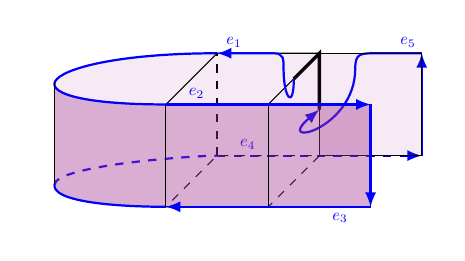
\begin{tikzpicture}[scale=1.3,every node/.style={scale=0.6}]
\clip (-2.1,-1) rectangle (1.9,1);

    \draw[blue,thick,-latex,dashed]
        (-0.25,-0.25) -- (1.75,-0.25) node[above,pos=0.15]{$e_4$};
    \draw[blue,thick,-latex]
        (1.75,-0.25) -- (1.75,0.75);
% B_1
    \draw[blue,thick,dashed]
        (-1.84,-0.54)  to[in=180,out=90,distance=0.2cm]
        (-0.25,-0.25);
    \fill[blue!45!red!80!white,fill opacity=0.4]
        (-0.75,0.25) to[out=180,in=-90,distance=0.2cm]
        (-1.84,0.47) --
         (-1.84,-0.54)  to[in=180,out=-90,distance=0.2cm]
         (-0.75,-0.75);
    \fill[blue!45!red!80!white,fill opacity=0.1,draw=blue,thick]
        (-0.25,0.75) to[out=180,in=180,distance=1.75cm] (-0.75,0.25);
    \draw
        (-1.84,-0.54) -- (-1.84,0.47);
    \draw[blue,thick]
        (-1.84,-0.54)  to[in=180,out=-90,distance=0.2cm]
        (-0.75,-0.75);
% ext region for B_1
    \draw[dashed]
        (-0.25,-0.25) rectangle (0.75,0.75);
    \draw[dashed]
        (-0.75,-0.75) -- (0.25,-0.75) -- 
        (0.75,-0.25) -- (-0.25,-0.25) -- (-0.75,-0.75);

    \fill[blue!45!red!80!white,fill opacity=0.1,draw=black]
        (-0.75,0.25) -- (0.25,0.25) -- 
        (0.75,0.75) -- (-0.25,0.75) -- (-0.75,0.25);

    \fill[blue!45!red!80!white,fill opacity=0.4,draw=black]
        (-0.75,-0.75) rectangle (0.25,0.25);

    \draw[very thick] (0.75,0.2) -- (0.75,0.75) -- (0.5,0.5) ;
% B_2

    \draw[blue,thick,latex-] 
        (0.75,0.2)  
        to[out=-140,in=-90,distance=0.6cm]
        (1.1,0.6) to[out=90,in=180,distance=0.15cm]
        (1.3,0.75) -- (1.75,0.75) node[above,pos=0.7]{$e_5$} ;
    \draw[blue,thick,-latex] 
        (0.5,0.5) to[out=-90,in=-90,distance=0.3cm] 
        (0.4,0.6) to[out=90,in=0,distance=0.1cm]
        (0.3,0.75) -- (-0.25,0.75) node[above,pos=0.7]{$e_1$} ; 

% ext region for B_2
    \fill[blue!45!red!80!white,fill opacity=0.1,draw=black]
        (0.75,-0.25) rectangle (1.75,0.75);
    % \draw[]
    %     (1.25,-0.75) -- 
    %     (1.75,-0.25) -- (0.75,-0.25);

    % \fill[blue!45!red!80!white,fill opacity=0,draw=black]
    %     (0.25,0.25) -- (1.25,0.25) -- 
    %     (1.75,0.75) -- (0.75,0.75) -- (0.25,0.25);
    \fill[blue!45!red!80!white,fill opacity=0.1]
        (0.25,0.25) -- (0.75,0.75) -- (0.75,0.25) --  (0.25,0.25);

    \fill[blue!45!red!80!white,fill opacity=0.4,draw=black]
        (0.25,-0.75) rectangle (1.25,0.25);
        
% 

    \draw[blue,thick,-latex]
        (-0.75,0.25) -- (1.25,0.25) node[above,pos=0.15]{$e_2$};
    \draw[blue,thick,-latex]
         (1.25,0.25) -- (1.25,-0.75);
    \draw[blue,thick,-latex]
        (1.25,-0.75) -- (-0.75,-0.75) node[below,pos=0.15]{$e_3$};

\end{tikzpicture}


\end{document}